\documentclass[a4paper,12pt]{article}
\usepackage[latin1]{inputenc}
%\usepackage[spanish]{babel}
\usepackage{amssymb}
\usepackage{graphicx}
%\usepackage{textcomp}
\usepackage{geometry}
\geometry{margin=1in}
\usepackage{cite}
\usepackage{url}
\usepackage{hyperref}
\usepackage{float}
\usepackage{amsmath}
\usepackage{cleveref}
\usepackage[autostyle=false]{csquotes}
\MakeOuterQuote{"}

\crefformat{footnote}{#2\footnotemark[#1]#3}

\title{\textbf{Project 2: Classical Planning}}
\author{Miguel Tasende}

%opening
\begin{document}


\maketitle

\section{Introduction}
The objective of this project is to build automatic players, with adversarial search techniques, to play the game "knights isolation".

\section{Initial Custom Player}
The initial player uses alpha-beta search with iterative deepening, and a simple heuristic. The heuristic function returns the total number of the player's free squares minus the total number of free squares of the opponent. That heuristic was shown in the course.\\
I run 100 matches with the "fair" flag activated: \\
\verb+(aind)$ python run_match -f -r 50 -o <OPPONENT> -p 4+.
The results for the initial player are shown below:\\

\begin{tabular}{|l|c|}
 \hline
Opponent & player wins\\
\hline
RANDOM & 98\% \\
\hline
GREEDY & 91\% \\
\hline
MINIMAX & 78\% \\
\hline
\end{tabular}


\section{Opening Book: Initial sampling}
An opening book was created. The data structure to save it is a python dictionary. The keys are the "state-action" pairs and the values are lists of two elements: the current estimated "state-action" value, and the current "number of visits" to that "state-action".\\
The book is filled by using the "\verb+game_history+" variable that is returned by the "play" function.

The initial sampling was deterministic and used some symmetries to add more samples to the states (horizontal, vertical and central symmetries were used). Symmetries are used only for the first two moves. The idea was to generate an initial sampling that covers all the "2-moves" states (all the possible first two moves) with at least some samples. All the depth-2 states were sampled 3 times, and each state has 3 symmetrical images, so each 2-moves state was sampled 9 times. The 1-move states were sampled 9 times, plus the times they appeared in other 2-moves starting states (a mechanism was implemented to add "move number 1" to the game history, given the "first 2 moves" state). That way the 1-move states were sampled: $9 + 98 * 3 * 3 = 891$ times.\\

From each starting state a custom vs custom player game is played. The custom player uses alpha-beta with iterative deepening.

\section{MCTS (not used in the final player)}
The MCTS algorithm was implemented. A first version was developed, that used a Node and a Tree class. In that version, every time a new node was expanded the node's state was searched in the tree and, if already existed, it was updated and a new parent was added (in that implementation nodes are in a 1-to-1 correspondence with states, and may have multiple parents). The backup process updates all the paths for all the parents.\\
A second, simplified version of MCTS was implemented that uses dictionaries as nodes, and doesn't allow for multiple parents (there may be more than one node representing the same state).\\
Both versions were tested with a random default policy and with "greedy players" for the default policy (with the same heuristic as used before).\\


The results were not too good. Some extra time for the moves was added but the improvements were not good enough. I think the problem is that the heuristics used are too simple, but more complicated ones (like simulating complete games with minimax or alpha-beta) would take too long to be practical. So, it was decided to use the MCTS algorithm, modified, to fill the opening book.

\section{Opening book: Sampling with MCTS}
A version of MCTS was created to store the actions of sampled games in a "\verb+game_history+" variable. The actions to be stored are those from the "tree policy" as well as those from the "default policy". That game history was used to create a new "\verb+tree_book+" with the same processing function as in the case of the deterministic sampling. The sampling in MCTS was decided with the UCT criterion.\\
The algorithm was run for several hours in different days (a mechanism to store the MCTS nodes and the book was implemented). For the "default policy" a game was played between two alpha-beta players with iterative deepening, that play as the initial (deterministically sampled) book in the first 2 moves (moves 3 and 4 don't have enough samples, so it is better not to use them, yet).
Finally, the initial book and the tree book were joined together in one large book (of depth 4).

\section{Results}
The player using the book in the first 4 moves ("book4") was compared against a player using random moves in the first 4 moves ("random4"). Both play like alpha-beta with iterative deepening after those moves.The results for 100 matches, without the "fair" flag, are below:\\
\verb+(aind)$ python run_match.py -r 50 -o <OPPONENT> -p 4+.\\

\begin{tabular}{|l|c|c|}
 \hline
Opponent & "random4" wins & "book4" wins\\
\hline
RANDOM & 93\% & 95\%\\
\hline
GREEDY & 88\% & 99\%\\
\hline
MINIMAX & 81\% & 92\%\\
\hline
\end{tabular}

The results seem to show an improvement. It is interesting to note that the book was created using a player similar to minimax, with a heuristic that is the same of the greedy player. That may explain that the player doesn't really improve much when playing against the RANDOM player (the book doesn't prepare the player for that... it may be not so expensive to add custom vs random games to the simulations to fill the book, but it wasn't done this time).

\subsection{Describe your process for collecting statistics to build your opening book. How did you choose states to sample? And how did you perform rollouts to determine a winner?}
The process was described in previous sections. First, a deterministic sampling up to depth 2, augmenting data with symmetries. The rollouts in that case were made using alpha-beta with iterative deepening (for both players).Then, running MCTS (with UCT) and recording the games to fill the book. The rollouts in that case were done the same way as before, but with the initial book added for the first 2 moves (the players are still alpha-beta with iterative deepening, but in the first two moves they use the book created from the deterministic sampling).

\subsection{What opening moves does your book suggest are most effective on an empty board for player 1 and what is player 2's best reply? }
A heatmap of the moves expected values can be seen below (the map represents the board image through a central symmetry):

\pagebreak
\begin{figure}[!h]
\centering
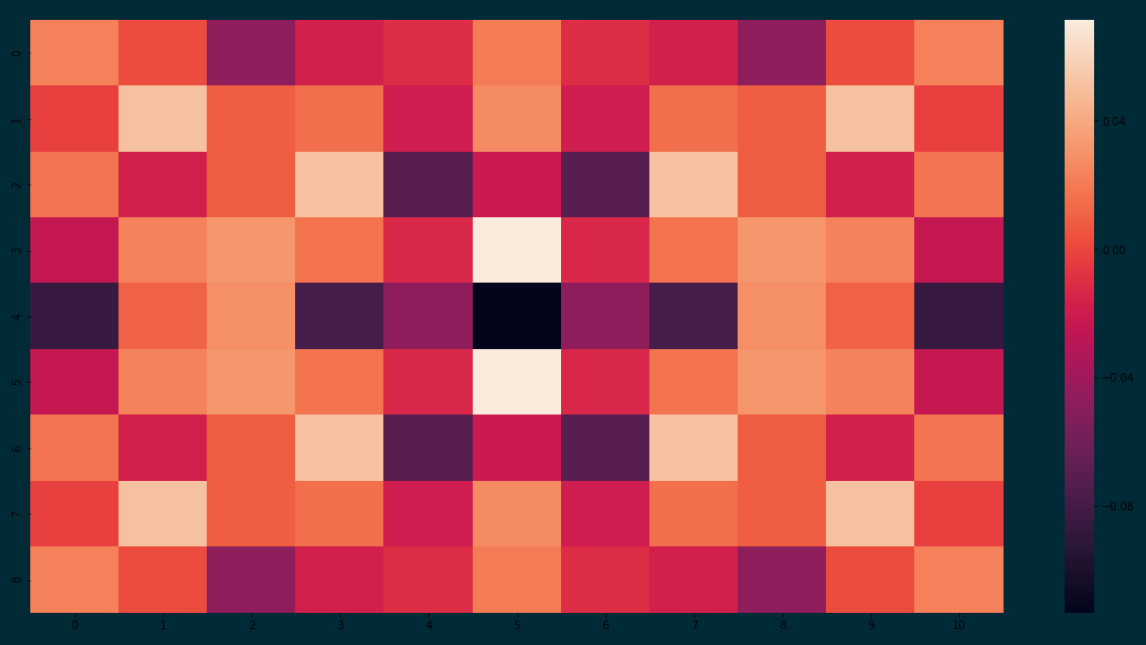
\includegraphics[width=5.0in]{first_move.png}
\caption{Heatmap with the expected values for the first move. The board is transformed by a central symmetry.}
\end{figure}

The moves that maximize the expected value are: 70 and 44. It can be seen that those are the ones immediately above and below the center of the board (DebugState was used to show that they correspond to the ones seen in the heatmap):

\begin{figure}[!h]
\centering
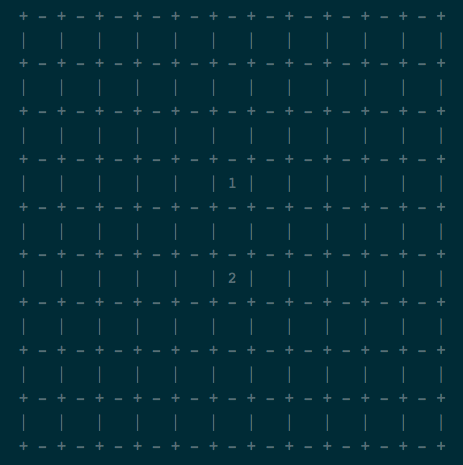
\includegraphics[width=3.0in]{best_first.png}
\caption{Result of printing the positions of the best moves in a DebugState board (just to check that they seem to be OK).}
\end{figure}

The best replies for player 2 if, for example, 70 is played (the other case is symmetrical), would be: 7, 79, 87, 3.\\
A heatmap for the best replies to first move = 70, can be seen below (the map represents the board image through a central symmetry).

\pagebreak
\begin{figure}[!h]
\centering
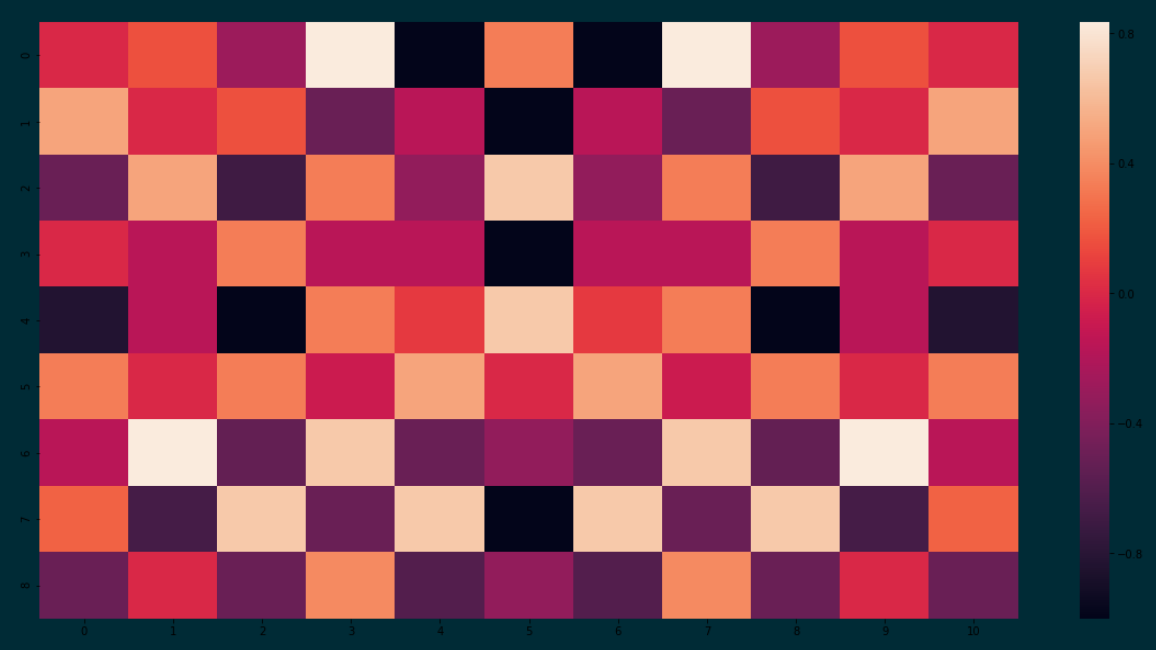
\includegraphics[width=5.0in]{second_move.png}
\caption{Heatmap with the expected values for the second move, if the first move is 70. The board is transformed by a central symmetry.}
\end{figure}

DebugState was used to check that the best replies correspond to what is seen in the heatmap (remember the heatmap shows the central symmetry of the board):

\pagebreak
\begin{figure}[!h]
\centering
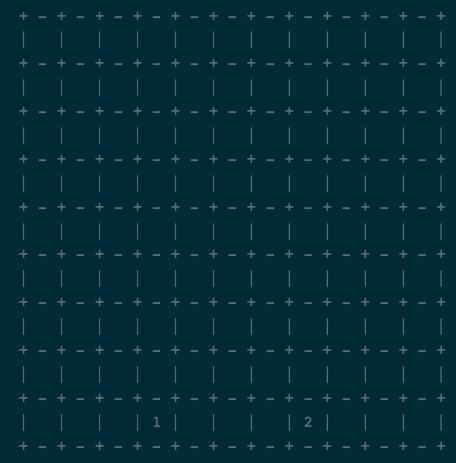
\includegraphics[width=3.0in]{best_second_a.png}
\caption{Result of printing the positions of two of the best second moves in a DebugState board (just to check that they seem to be OK).}
\end{figure}

\begin{figure}[!h]
\centering
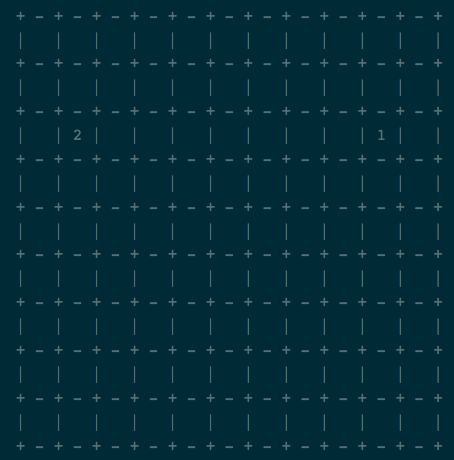
\includegraphics[width=3.0in]{best_second_b.png}
\caption{Result of printing the positions of the other two best second moves in a DebugState board (just to check that they seem to be OK).}
\end{figure}

After taking into account the central symmetry, everything seems to be OK.

\end{document}